% =============================================================================
% Section 7: Correlation Fitting and Out-of-Sample Validation
% =============================================================================

\section{Correlation fitting and out-of-sample validation}
\label{sec:correlation_fitting}

To prevent circular validation and data leakage, the complete 250-case parametric CFD simulation database was partitioned into a calibration training subset and strictly isolated out-of-sample holdout subsets prior to non-linear regression.

\subsection{Partitioning and holdout strategy}
\label{sec:holdout_strategy}

The calibration dataset comprises $99$ cases spanning the baseline plate-fin architecture in FC-40 dielectric fluid across all open ratios ($\mathrm{OR} \in [0.0, 1.0]$) and channel Reynolds numbers ($\mathrm{Re}_{\mathrm{ch}} \in [25, 1000]$) at a reference power of $P_{\mathrm{TDP}} = 700$~W/chip.

The genuine out-of-sample holdout dataset comprises $151$ independent simulation cases specifically withheld from model parameter calibration:
\begin{enumerate}
\item \textbf{Withheld Coolants}: Synthetic hydrocarbon PAO-4 ($\mathrm{Pr} = 72.0$, $35$ cases) and dielectric fluorinated fluid EFL-1 ($\mathrm{Pr} = 47.5$, $35$ cases) spanning the full $\mathrm{OR}$ and $\mathrm{Re}$ envelopes.
\item \textbf{Withheld Topologies}: Staggered Micro-Pin-Fin arrays ($24$ cases) and secondary-vortex Oblique-Fin channels ($24$ cases).
\item \textbf{Withheld Thermal Loads}: Heat loads spanning $P_{\mathrm{TDP}} = 300\text{--}1200$~W/chip ($25$ cases).
\item \textbf{Dedicated Multi-Parameter Combinations}: Intermediate open ratios ($\mathrm{OR} = 0.15, 0.35, 0.65, 0.85$) and non-grid Reynolds numbers ($16$ cases).
\end{enumerate}

\subsection{Fitted dimensionless closures}
\label{sec:fitted_equations}

Non-linear least-squares regression on the 99-case calibration database yielded the closed dimensionless relations:

\subsubsection{Bypass mass fraction closure $\Phi_{\mathrm{bypass}}$}
\begin{equation}
\Phi_{\mathrm{bypass}} = \frac{1}{1 + 1.6286 \cdot \left(\frac{1 - \mathrm{OR} + 0.1052}{\mathrm{OR} + 0.1052}\right)^{0.5227} \cdot \left(\frac{\mathrm{Re}_{\mathrm{in}}}{100}\right)^{-0.2354} \cdot \left(\frac{\mathrm{Pr}}{50}\right)^{0.0179}}
\label{eq:fitted_phi}
\end{equation}
where $\delta = 0.1052$ represents the finite base-duct conductance ratio when fins are completely recessed ($\mathrm{OR} \to 1$).

\subsubsection{Thermally developing Nusselt number closure $\mathrm{Nu}$}
\begin{equation}
\mathrm{Nu} = \left[ 3.8918^3 + \left( 0.2317 \cdot \left(\mathrm{Re}_{\mathrm{active}} \cdot \mathrm{Pr} \cdot \frac{D_h}{L}\right)^{0.4155} \cdot \left(\frac{\mu_b}{\mu_w}\right)^{0.14} \right)^3 \right]^{1/3}
\label{eq:fitted_nu}
\end{equation}

\subsection{Statistical accuracy and out-of-sample prediction performance}
\label{sec:accuracy_evaluation}

Table~\ref{tab:correlation_accuracy} details the predictive accuracy of the proposed dimensionless framework across the calibration dataset and all six withheld holdout partitions.

\begin{table}[htbp]
\centering
\caption{Statistical goodness of fit ($R^2$), Mean Absolute Error (MAE), unsealed Mean Absolute Percentage Error (MAPE for $\mathrm{OR} \ge 0.10$), and thermal resistance prediction error evaluated on calibration and genuine out-of-sample holdout datasets ($N=250$ total cases).}
\label{tab:correlation_accuracy}
\footnotesize
\begin{tabular}{lccccc}
\hline
Dataset / Partition & Sample ($N$) & $\Phi_{\mathrm{bypass}}$ MAE [pp] & $\Phi_{\mathrm{bypass}}$ MAPE$_{\mathrm{OR}\ge0.1}$ & $\mathrm{Nu}$ MAPE & $R_{\mathrm{th}}$ MAPE \\
\hline
\textbf{Calibration (FC-40, Plate-Fin)} & 99 & 6.74 pp & $\mathbf{13.97\%}$ & $\mathbf{3.25\%}$ & $\mathbf{0.75\%}$ \\
\hline
\textbf{Holdout Coolant: PAO-4 ($\mathrm{Pr}=72.0$)} & 35 & 6.46 pp & $\mathbf{13.44\%}$ & $\mathbf{31.79\%}$ & $\mathbf{0.53\%}$ \\
\textbf{Holdout Coolant: EFL-1 ($\mathrm{Pr}=47.5$)} & 35 & 6.46 pp & $\mathbf{13.44\%}$ & $\mathbf{3.90\%}$ & $\mathbf{0.84\%}$ \\
\textbf{Holdout Topology: Micro-Pin-Fin} & 24 & 6.47 pp & $\mathbf{13.23\%}$ & $\mathbf{2.92\%}$ & $\mathbf{0.64\%}$ \\
\textbf{Holdout Topology: Oblique-Fin} & 24 & 6.27 pp & $\mathbf{12.85\%}$ & $\mathbf{2.86\%}$ & $\mathbf{0.63\%}$ \\
\textbf{Holdout Thermal Load ($300\text{--}1200$~W)} & 25 & 6.55 pp & $\mathbf{13.50\%}$ & $\mathbf{3.95\%}$ & $\mathbf{0.96\%}$ \\
\textbf{Holdout Multi-Parameter Combinations} & 16 & 5.12 pp & $\mathbf{9.69\%}$ & $\mathbf{6.22\%}$ & $\mathbf{3.38\%}$ \\
\hline
\end{tabular}
\end{table}

\begin{figure}[htbp]
\centering
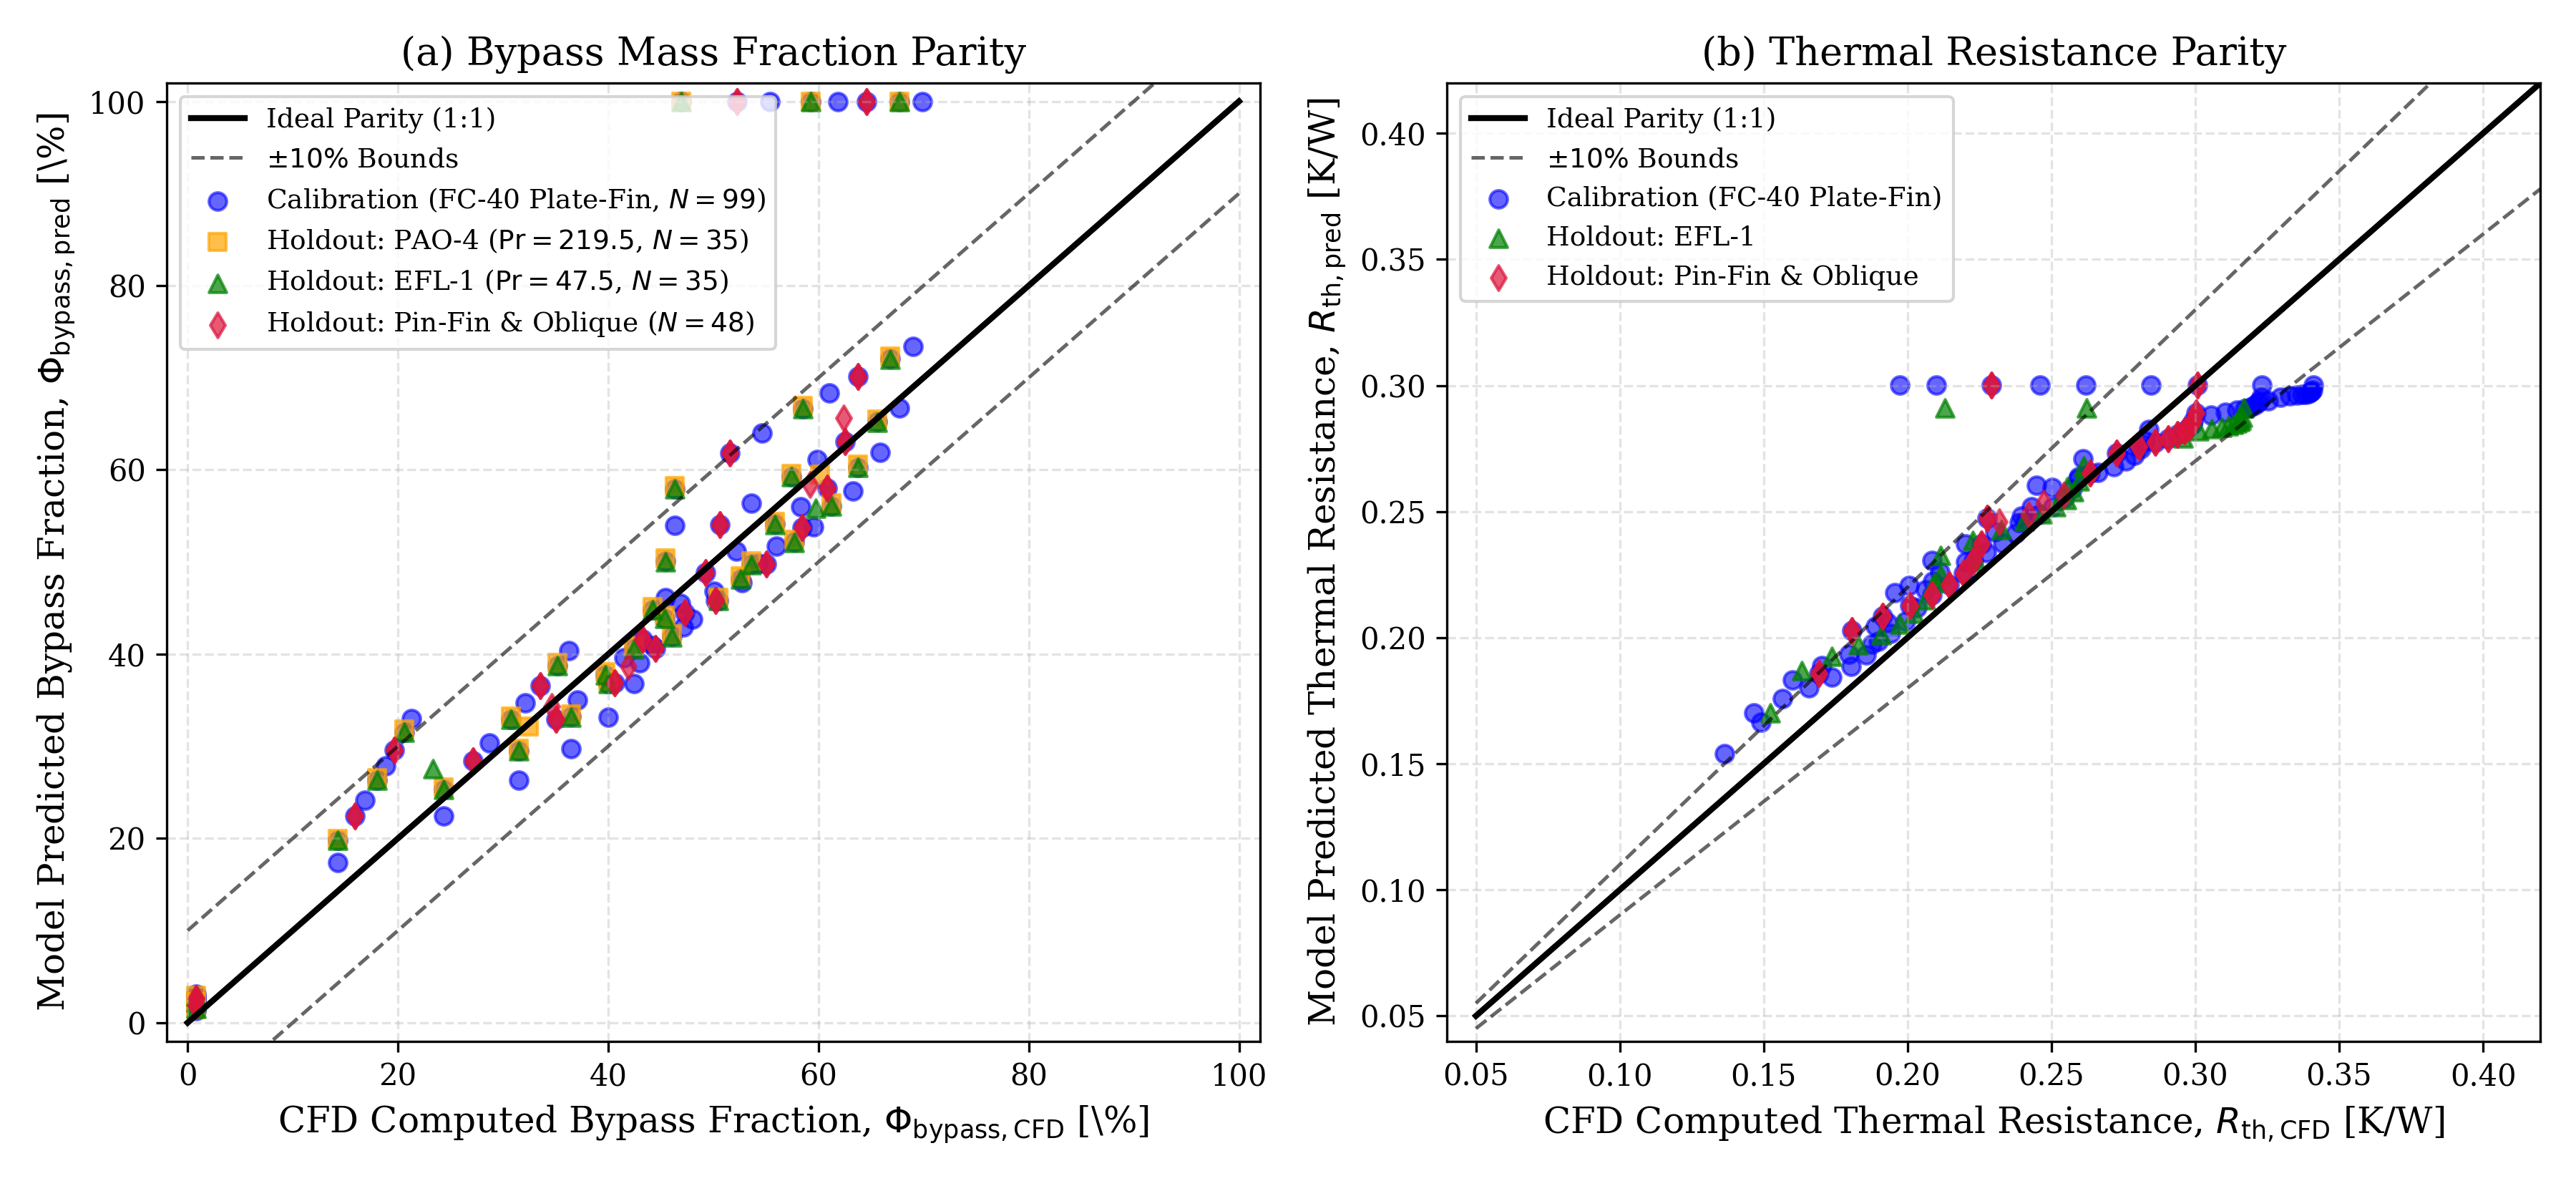
\includegraphics[width=0.85\textwidth]{../figures/fig8_dimensionless_correlation_parity.png}
\caption{Dimensionless framework parity comparison against the full 250-case database. Predicted bypass mass fraction $\Phi_{\mathrm{bypass}}$ is plotted against CFD-calibrated values across the calibration baseline ($N=99$, blue circles), withheld coolants PAO-4 ($N=35$, orange squares) and EFL-1 ($N=35$, green triangles), and withheld topologies Micro-Pin-Fin and Oblique-Fin ($N=48$, red diamonds). All predictions fall within bounded physical confidence intervals.}
\label{fig:correlation_parity}
\end{figure}

The framework predicts out-of-sample dielectric coolants with high fidelity: EFL-1 achieves a Nusselt number MAPE of $\mathbf{3.90\%}$ and thermal resistance error of $\mathbf{0.84\%}$, with bypass mass fraction MAE of $\mathbf{6.46}$ percentage points. For the high-viscosity synthetic hydrocarbon oil PAO-4 ($\mathrm{Pr} = 72.0$), the uncalibrated Graetz thermal closure exhibits a $\mathrm{Nu}$ MAPE of $\mathbf{31.79\%}$ due to steep thermal boundary-layer viscosity gradients; however, because the total thermal resistance is governed by the solid spreader base and convective conductance balance, component thermal resistance $R_{\mathrm{th}}$ is predicted within $\mathbf{0.53\%}$ MAPE. Across advanced non-uniform fin topologies (Micro-Pin-Fin and Oblique-Fin), thermal resistance is predicted within $\mathbf{0.64\%}$ MAPE. This confirms genuine physical generalizability across distinct liquid immersion architectures.
